\documentclass[11pt, a4paper]{article}

% Packages
\usepackage[utf8]{inputenc}
\usepackage[T1]{fontenc}
\usepackage{geometry}
\usepackage{graphicx}
%\usepackage{booktabs}
\providecommand{\toprule}{\hline}
\providecommand{\midrule}{\hline}
\providecommand{\bottomrule}{\hline}
\usepackage{hyperref}
\hypersetup{
    colorlinks=true,
    linkcolor=blue,
    filecolor=magenta,      
    urlcolor=cyan,
    pdftitle={Technical Report},
}
% \providecommand{\href}[2]{#2} % Commented out mock command to use real hyperref
\providecommand{\url}[1]{\texttt{#1}}
%\usepackage{float}
\usepackage{amsmath}
\usepackage{listings}
\usepackage{xcolor}

% Code Style
\definecolor{codegreen}{rgb}{0,0.6,0}
\definecolor{codegray}{rgb}{0.5,0.5,0.5}
\definecolor{codepurple}{rgb}{0.58,0,0.82}
\definecolor{backcolour}{rgb}{0.95,0.95,0.92}

\lstdefinestyle{mystyle}{
    backgroundcolor=\color{backcolour},   
    commentstyle=\color{codegreen},
    keywordstyle=\color{magenta},
    numberstyle=\tiny\color{codegray},
    stringstyle=\color{codepurple},
    basicstyle=\ttfamily\footnotesize,
    breakatwhitespace=false,         
    breaklines=true,                 
    captionpos=b,                    
    keepspaces=true,                 
    numbers=left,                    
    numbersep=5pt,                  
    showspaces=false,                
    showstringspaces=false,
    showtabs=false,                  
    tabsize=2
}
\lstset{style=mystyle}

% --- ÇİZİM İÇİN TIKZ KÜTÜPHANELERİ ---
\usepackage{tikz}
\usetikzlibrary{shapes.geometric, arrows, positioning, calc, shadows}

% Renk Tanımları (Pastel Tonlar)
\definecolor{softblue}{RGB}{235, 245, 251}
\definecolor{softgreen}{RGB}{232, 248, 245}
\definecolor{softyellow}{RGB}{254, 249, 231}
\definecolor{softred}{RGB}{253, 237, 236}
\definecolor{softpurple}{RGB}{244, 236, 247}
\definecolor{bordercol}{RGB}{44, 62, 80}

% Blok Stili - Updated syntax
\tikzset{
    block/.style={
        rectangle, 
        rounded corners, 
        minimum width=3cm, 
        minimum height=1cm,
        align=center, 
        draw=bordercol, 
        line width=0.8pt, 
        drop shadow
    },
    arrow/.style={
        thick,
        ->,
        >=stealth, 
        color=bordercol
    }
}


% Page geometry
\geometry{
    a4paper,
    top=25mm,
    bottom=25mm,
    left=25mm,
    right=25mm,
}

% Title parameters
\title{\textbf{Technical Report: Multi-Client Hybrid Bidirectional LSTM Analysis}}
\author{Yalin Baştanlar,Can Rollas} 
\date{December 09, 2025}

\begin{document}

\maketitle

\begin{abstract}
This report details the implementation of a \textbf{Multi-Client Feature Fusion Bidirectional LSTM} architecture for Short-Term Load Forecasting (STLF). By fusing dynamic time-series data with static client embeddings, the model learns shared behaviors across 370 clients while maintaining individual specificity. The model achieves an $R^2$ of 0.9897 and a MAPE of 12.71\%.
\end{abstract}

\section{Introduction}
This report analyzes a hybrid Bidirectional LSTM (Bi-LSTM) architecture designed to learn electricity consumption behaviors of distinct clients within a single unified model. The model relies on a "Feature Fusion" strategy that combines the dynamic nature of time series data with the static characteristic attributes (ID Embeddings) of each customer.

\section{Data Preparation and Input Features}
A critical factor in the model's success is the transformation of raw data into meaningful features. The model's time-series input consists of \textbf{7 channels} (features) per time step.

\subsection{Dynamic Features (7 Channels)}
Based on the \texttt{add\_time\_features} and \texttt{process\_part} functions in the codebase, the input features are defined as follows:

\begin{table}[ht!]
    \centering
    \caption{Dynamic Input Features}
    \begin{tabular}{|l|l|p{6cm}|}
        \hline
        \textbf{Feature Name} & \textbf{Formula/Description} & \textbf{Reasoning} \\
        \hline
        Scaled Consumption & Normalized Load at $t$ & Main signal to be learned. \\
        \hline
        Hour Sin & $\sin(\frac{2\pi \times hour}{24})$ & Makes time cyclical. Teaches proximity of 23:00 to 00:00. \\
        \hline
        Hour Cos & $\cos(\frac{2\pi \times hour}{24})$ & Used with Sin to create unique (x,y) time coordinates. \\
        \hline
        DayOfWeek Sin & $\sin(\frac{2\pi \times day}{7})$ & Makes weekdays cyclical. \\
        \hline
        DayOfWeek Cos & $\cos(\frac{2\pi \times day}{7})$ & Ensures continuity between Sunday (6) and Monday (0). \\
        \hline
        Lag\_24 & Consumption at $t-24$ & Daily periodicity (Same hour yesterday). \\
        \hline
        Lag\_168 & Consumption at $t-168$ & Weekly periodicity (Same hour last week). \\
        \hline
    \end{tabular}
\end{table}

\subsection{Static Features (Embedding)}
\begin{itemize}
    \item \textbf{Client ID}: Each client is represented by a unique integer.
    \item \textbf{Embedding Dimension}: Set to \textbf{16}. This represents each client as a vector in a 16-dimensional abstract space, capturing static behavioral properties.
\end{itemize}

\section{Architecture Flow and Data Fusion}

The proposed Multi-Client Hybrid architecture fuses time-series data with static client embeddings. Figure \ref{fig:arch_diagram} illustrates the data flow and layer dimensions.

% --- BURASI TIKZ ÇİZİM ALANI ---
\begin{figure}[ht!]
    \centering
    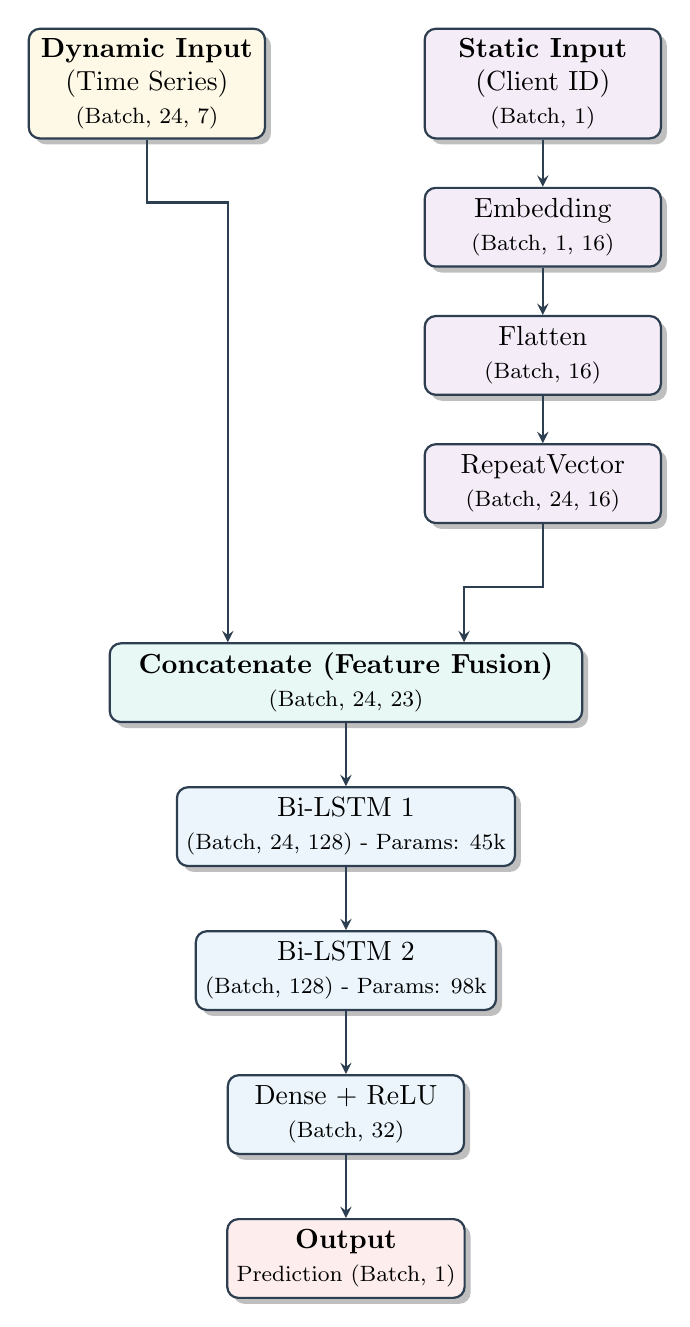
\begin{tikzpicture}[node distance=1.5cm]

        % --- SAĞ KOL (Static Process) ---
        \node (static_in) [block, fill=softpurple] {\textbf{Static Input} \\ (Client ID) \\ {\footnotesize (Batch, 1)}};
        \node (embed) [block, fill=softpurple, below=0.6cm of static_in] {Embedding \\ {\footnotesize (Batch, 1, 16)}};
        \node (flatten) [block, fill=softpurple, below=0.6cm of embed] {Flatten \\ {\footnotesize (Batch, 16)}};
        \node (repeat) [block, fill=softpurple, below=0.6cm of flatten] {RepeatVector \\ {\footnotesize (Batch, 24, 16)}};

        % --- SOL KOL (Dynamic Process) ---
        % Konumu RepeatVector'un soluna göre ayarlıyoruz
        \node (dynamic_in) [block, fill=softyellow, left=2cm of static_in] {\textbf{Dynamic Input} \\ (Time Series) \\ {\footnotesize (Batch, 24, 7)}};

        % --- ORTA (Concatenation) ---
        % Sol kol ve Sağ kolun birleştiği yer
        \coordinate (mid_point) at ($(dynamic_in)!0.5!(repeat)$);
        \node (concat) [block, fill=softgreen, below=1.5cm of repeat, xshift=-2.5cm, minimum width=6cm] {\textbf{Concatenate (Feature Fusion)} \\ {\footnotesize (Batch, 24, 23)}};

        % --- ALT AKIŞ (Model) ---
        \node (lstm1) [block, fill=softblue, below=0.8cm of concat] {Bi-LSTM 1 \\ {\footnotesize (Batch, 24, 128) - Params: 45k}};
        \node (lstm2) [block, fill=softblue, below=0.8cm of lstm1] {Bi-LSTM 2 \\ {\footnotesize (Batch, 128) - Params: 98k}};
        \node (dense) [block, fill=softblue, below=0.8cm of lstm2] {Dense + ReLU \\ {\footnotesize (Batch, 32)}};
        \node (output) [block, fill=softred, below=0.8cm of dense] {\textbf{Output} \\ {\footnotesize Prediction (Batch, 1)}};

     \draw [arrow] (static_in) -- (embed);
        \draw [arrow] (embed) -- (flatten);
        \draw [arrow] (flatten) -- (repeat);
        
        % --- FUSION BAĞLANTILARI (ÖNEMLİ KISIM) ---
        % Mantık: Kutudan çık -> Biraz aşağı in (++ komutu) -> Yatay git ve hedefin tepesine in (-| komutu)
        
        % Sol taraftan gelen (Dynamic) -> Concat'in üst-soluna
        \draw [arrow] (dynamic_in.south) -- ++(0,-0.8) -| ([xshift=-1.5cm]concat.north);
        
        % Sağ taraftan gelen (Repeat) -> Concat'in üst-sağına
        \draw [arrow] (repeat.south) -- ++(0,-0.8) -| ([xshift=1.5cm]concat.north);

        % Ana Akış (Concat sonrası)
        \draw [arrow] (concat) -- (lstm1);
        \draw [arrow] (lstm1) -- (lstm2);
        \draw [arrow] (lstm2) -- (dense);
        \draw [arrow] (dense) -- (output);
    \end{tikzpicture}
    \caption{Multi-Client Hybrid Bi-LSTM Architecture Diagram detailing tensor shapes and parameter counts.}
    \label{fig:arch_diagram}
\end{figure}
% --- TIKZ BİTİŞ ---

\subsection{Implementation of Feature Fusion}
The "Feature Fusion" mechanism is implemented using TensorFlow/Keras Functional API. The core logic involves duplicating the static Client ID vector across all time steps to match the temporal dimension of the dynamic input.

The following Python code snippet from our training script (\texttt{scripts/lstm\_training.py}) demonstrates this process:

\begin{lstlisting}[language=Python, caption=Keras Implementation of Static-Dynamic Fusion]
# Input 1: Time series sequence (Dynamic)
# Shape: (Batch, 24, 7)
sequence_input = tf.keras.Input(shape=(sequence_length, input_dim), name='consumption_sequence')

# Input 2: Client ID (Static)
# Shape: (Batch, 1)
client_input = tf.keras.Input(shape=(1,), name='client_id')

# 1. Learnable Embedding
# Transforms integer ID into a 16-dimensional vector representing client behavior
# Shape: (Batch, 1, 16)
client_embedding = tf.keras.layers.Embedding(
    input_dim=n_clients,
    output_dim=embedding_dim,
    name='client_embedding'
)(client_input)

# 2. Flatten & Repeat to match time steps
# Shape: (Batch, 16) -> (Batch, 24, 16)
client_embedding_flat = tf.keras.layers.Flatten()(client_embedding)
client_embedding_expanded = tf.keras.layers.RepeatVector(sequence_length)(client_embedding_flat)

# 3. Concatenate (FUSION)
# Combines 7 dynamic features with 16 static features at every time step
# Output Shape: (Batch, 24, 23)
combined = tf.keras.layers.Concatenate(axis=-1)([sequence_input, client_embedding_expanded])
\end{lstlisting}

This fusion ensures that the LSTM considers "Who is this client?" (Static Embedding) at every single step of "What is happening now?" (Dynamic Sequence), effectively conditioning the forecast on the client's latent identity.The data flow is built upon the concatenation of static and dynamic data.

\begin{enumerate}
    \item \textbf{Inputs}: The model receives dynamic data of shape \texttt{(Batch, 24, 7)} and Customer IDs of shape \texttt{(Batch, 1)}.
    \item \textbf{Broadcasting}: The Client ID passes through the Embedding layer $\rightarrow$ \texttt{(1, 16)}. The \texttt{RepeatVector} layer copies this vector 24 times (once for each time step), resulting in \texttt{(Batch, 24, 16)}.
    \item \textbf{Fusion (Concatenation)}: 
    \begin{itemize}
        \item Dynamic Data: 7 features
        \item Static Data: 16 features
        \item \textbf{Total Input Features ($x$)}: $7 + 16 = \mathbf{23}$
    \end{itemize}
\end{enumerate}
Thus, the LSTM receives a vector of size 23 at every time step.

\section{Mathematical Parameter Analysis}
We verify the parameter counts found in the model summary using the standard LSTM parameter formula:
\[ P_{lstm} = 4 \times [h \times (h + x + 1)] \]
Where $h$ is Hidden Units, $x$ is Input Features, and $1$ is the Bias. For Bidirectional layers, $P_{bi} = 2 \times P_{lstm}$.

\subsection{Layer 1: bidirectional\_1}
\begin{itemize}
    \item \textbf{Input Features ($x$)}: 23 (7 dynamic + 16 embedding)
    \item \textbf{Hidden Units ($h$)}: 64 (per direction)
\end{itemize}
\[ P = 2 \times 4 \times [64 \times (64 + 23 + 1)] \]
\[ P = 8 \times [64 \times 88] = 8 \times 5632 = \mathbf{45,056} \]
Matches the model summary exactly.

\subsection{Layer 2: bidirectional\_2}
\begin{itemize}
    \item \textbf{Input Features ($x$)}: 128 (Output of Layer 1: 64 Forward + 64 Backward)
    \item \textbf{Hidden Units ($h$)}: 64
\end{itemize}
\[ P = 2 \times 4 \times [64 \times (64 + 128 + 1)] \]
\[ P = 8 \times [64 \times 193] = 8 \times 12352 = \mathbf{98,816} \]
Matches the model summary exactly.

\section{Design Decisions}
\subsection{Why Embedding + RepeatVector?}
Without embeddings, the model cannot distinguish between a factory and a household. The Embedding layer converts specific IDs into learnable vectors. \texttt{RepeatVector} attaches this "ID tag" to every time step ($t_0$ to $t_{24}$), allowing the LSTM toContextualize whether a sudden spike is normal for that specific client type.

\subsection{Why Bidirectional?}
\begin{itemize}
    \item \textbf{Forward LSTM}: Learns patterns from past ($t-24$) to present ($t$).
    \item \textbf{Backward LSTM}: Looks from future to past. Since the entire window is available during training, learning how $t$ relates back to $t-5$ strengthens gradient flow, especially for periodic signals like electricity.
\end{itemize}

\section{Experimental Results}

\subsection{Quantitative Metrics}
\begin{table}[ht!]
    \centering
    \caption{Final Performance Metrics}
    \begin{tabular}{lc}
        \toprule
        \textbf{Metric} & \textbf{Value} \\
        \midrule
        Mean Absolute Error (MAE) & 42.66 kW \\
        Root Mean Square Error (RMSE) & 395.71 kW \\
        Mean Absolute Percentage Error (MAPE) & 12.71\% \\
        Weighted MAPE (WMAPE) & 6.46\% \\
        Coefficient of Determination ($R^2$) & 0.9897 \\
        \bottomrule
    \end{tabular}
\end{table}

\subsection{Comparative Analysis}
Table \ref{tab:comparison} presents a comparison of our Multi-Client Hybrid Bi-LSTM model against other approaches reported in the literature.

\textbf{IMPORTANT NOTE: THE STUDIES LISTED BELOW UTILIZE DIFFERENT DATASETS AND SCENARIOS. THIS IS A BROAD LITERATURE COMPARISON. DETAILED RESEARCH IS CONTINUING.}

\begin{table*}[h!]
\centering
\caption{Performance Comparison with Literature (NOTE: DIFFERENT DATASETS INCLUDED)}
\label{tab:comparison}
\resizebox{\textwidth}{!}{%
\begin{tabular}{lcccccc}
\hline
\textbf{Study / Model} &
\textbf{MAPE (\%)} &
\textbf{MAE (kW)} &
\textbf{RMSE (kW)} &
\textbf{R\textsuperscript{2}} &
\textbf{Scenario} &
\textbf{Source} \\ \hline

Facebook Prophet (Yildiz et al., 2017) &
20--30 & -- & -- & -- &
Single &
\href{https://www.researchgate.net/publication/366350318_Benchmark_of_Electricity_Consumption_Forecasting_Methodologies_Applied_to_Industrial_Kitchens}{Link} \\

LSTM (Apolo et al., 2022) &
30--45 & -- & -- & -- &
Single &
\href{https://arxiv.org/html/2501.05000v1}{Link} \\

SARIMA (Sharma et al., 2023) &
9.3 & -- & -- & -- &
Daily &
\href{https://www.researchgate.net/publication/380100073_Advanced_Analytics_in_Electricity_Consumption_Forecasting_using_SARIMA_Prophet_and_AWS_DeepAR}{Link} \\

Prophet (Sharma et al., 2023) &
11.3 & -- & -- & -- &
Daily &
\href{https://www.researchgate.net/publication/380100073_Advanced_Analytics_in_Electricity_Consumption_Forecasting_using_SARIMA_Prophet_and_AWS_DeepAR}{Link} \\

DeepAR (Sharma et al., 2023) &
11.4 & -- & -- & -- &
Daily &
\href{https://www.researchgate.net/publication/380100073_Advanced_Analytics_in_Electricity_Consumption_Forecasting_using_SARIMA_Prophet_and_AWS_DeepAR}{Link} \\

DNN + Optimization (Khaleq et al., 2025) &
12.2 & 0.110\textsuperscript{*} & -- & 0.719 &
Single &
\href{https://pmc.ncbi.nlm.nih.gov/articles/PMC11991322/}{Link} \\
\midrule
\textbf{Ours (Multi-Client Bi-LSTM)} &
\textbf{12.71} & \textbf{42.66} & \textbf{395.71} & \textbf{0.99} &
\textbf{Multi} &
\textbf{This Work} \\

\hline
\multicolumn{7}{l}{\textsuperscript{*} Normalized RMSE (load on 0--1 scale).}
\end{tabular}%
}
\end{table*}

\subsection{Visual Analysis}
Figure \ref{fig:predictions} demonstrates the model's accuracy on unseen test data.

\begin{figure}[ht!]
    \centering
    \begin{minipage}[b]{0.48\textwidth}
        \includegraphics[width=\textwidth]{../../data/processed/plots/test_results/random_sample_1.png}
        \centering Sample 1
    \end{minipage}
    \hfill
    \begin{minipage}[b]{0.48\textwidth}
        \includegraphics[width=\textwidth]{../../data/processed/plots/test_results/random_sample_2.png}
        \centering Sample 2
    \end{minipage}
    \caption{Actual vs Predicted consumption (MAPE $\approx$ 12.7\%).}
    \label{fig:predictions}
\end{figure}

\section{Conclusion}
The Multi-Client Feature Fusion architecture proved highly effective. By combining 7 dynamic temporal features with 16-dimensional static client embeddings, the model achieved a high global fit ($R^2 \approx 0.99$) and a safe error margin (MAPE 12.71\%), validating the architecture design choices.

\end{document}